\documentclass[a4paper,12pt,twoside]{book}
\usepackage{graphicx}
\usepackage{natbib}
\graphicspath{ {figures/} }
\usepackage{array}
\usepackage{lipsum}
\usepackage{float}
\usepackage{siunitx}
\usepackage{ xcolor}
\usepackage[T1]{fontenc}
\usepackage[utf8]{inputenc}
\usepackage[left=2.5cm,right=2.5cm,top=3cm,bottom=3cm]{geometry}
\tolerance=1
\emergencystretch=\maxdimen
\hyphenpenalty=10000
\hbadness=10000
\usepackage[belowskip=-10pt,aboveskip=10 pt]{caption}
\usepackage{setspace}
\def\bibfont{\footnotesize}
\doublespacing
\setlength{\intextsep}{20pt plus 2pt minus 2pt}
\setlength{\belowcaptionskip}{-15pt}

\usepackage{natbib}
\raggedbottom

\usepackage[french]{babel}
%\usepackage{lastpage}
\usepackage{fancyhdr}
\pagestyle{fancy}
\renewcommand{\headrulewidth}{2pt}
\renewcommand{\footrulewidth}{1pt}

\fancyhf{}
\renewcommand{\chaptermark}[1]{\markboth{\bsc{\chaptername~\thechapter{} :} #1}{}}
\renewcommand{\sectionmark}[1]{\markright{\thesection{} \ #1}}
\renewcommand{\headrulewidth}{0pt}
\lhead[\textsl{\leftmark}]{\textsl{\rightmark}}
\rhead[\textsl{\rightmark}]{\textsl{\leftmark}}
\cfoot[\thepage]{\thepage}
\setlength{\headheight}{15pt}

\DeclareDocumentCommand{\corr}{m}{{\color{red}#1}}
\DeclareDocumentCommand{\corrg}{m}{{\color{teal}#1}}
\renewcommand{\headrulewidth}{2pt}
\renewcommand{\footrulewidth}{1pt}
\begin{document}
	
	%	\frontmatter
	%	\input{Chaps/Dedicace.tex}
	%\input{Chaps/Dedicace1.tex}
	%	\input{Chaps/Remer.tex}
		%\	tableofcontents
		%\listoffigures
	%	\listoftables
	%	\mainmatter
		%\markboth{INTRODUCTION}{}
	%	\input{Chaps/Intro.tex}
	%	
\chapter{État de l'art }



\section*{Introduction }
Dans ce chapitre, nous nous penchons sur les fondements de la connectivité réseau en étudiant les technologies établies telles que les MPLS et les VPNs . Nous examinons leurs fonctionnements et leurs architectures. En outre, nous abordons les défis rencontrés, en particulier en termes de flexibilité et de coût. Enfin, nous introduisons la solution SD-WAN comme une alternative prometteuse pour répondre aux besoins évolutifs des réseaux modernes.

\section{Etudes de l'éxistant }
\subsection{Mpls }
\subsubsection{Généralité sur mpls }
\begin{itemize}
	\item[$\bullet$]\textbf{Définition:} 
	
	MPLS, acronyme de Multiprotocol Label Switching, a été initialement introduit dans les années 1970 par plusieurs ingénieurs Internet pour résoudre diverses problématiques d'Internet, principalement en ce qui concerne les performances de routage, dans lesquelles l'en-tête de chaque paquet devait être lu et analysé avant d'être envoyé vers la bonne destination. Après près de 20 ans de lutte et de développement, MPLS a finalement été reconnu et confirmé par l'IETF (Internet Engineering Task Force) à la fin des années 1990, devenant ainsi une norme ouverte prête à être adoptée. De plus en plus adoptée par les fournisseurs de services dans leurs infrastructures principales, MPLS s'intègre aux protocoles de couche 2 et de couche 3.

\end{itemize}
\begin{itemize}
	\item[$\bullet$]\textbf{L'en-tête MPLS :} 
	
L'en-tête MPLS a une longueur de 32 bits comme montre la figure.
\begin{figure} [H]
	\begin{center}
		\centering
		\hspace*{-0.5cm}
		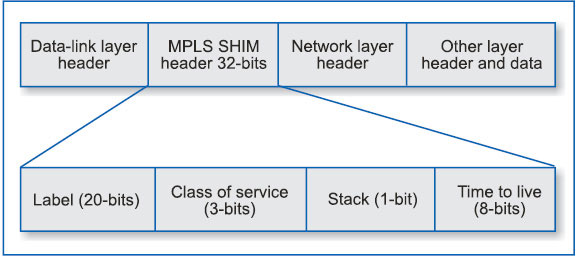
\includegraphics[width=0.67\linewidth]{Images/mpls entete}
	\end{center}
	\caption{Entête MPLS}
\end{figure} 

Le champ d'étiquette est de 20 bits, et ces étiquettes sont attachées aux paquets au point d'entrée dans un réseau MPLS. 

Dans le réseau, les étiquettes sont utilisées pour router les paquets sans tenir compte des informations d'en-tête originales des paquets. Elles peuvent être empilées comme une pile LIFO, ce qui permet à MPLS d'être utilisé pour le transport et la distribution.

Le champ CoS (Class of Service) est de 3 bits. Il affecte les algorithmes de planification et/ou de suppression appliqués au paquet lors de sa transmission à travers le réseau. Ces bits ne sont pas modifiés par l'implémentation embarquée de MPLS.
Le bit Stack est défini à 1 pour la dernière entrée dans la pile d'étiquettes et à 0 pour toutes les autres entrées de pile d'étiquettes.

Le champ TTL (Time To Live) est de 8 bits. Il est décrémenté de 1 chaque fois que le paquet passe par un routeur. Le paquet est supprimé lorsque le TTL atteint zéro. 
	
\end{itemize}
\subsubsection{Architecture d'un réseau MPLS de base }
C’est une architecture qui fait référence à une mise en œuvre simple et directe de MPLS, où les routeurs MPLS sont utilisés pour acheminer les paquets en fonction des étiquettes MPLS sans ajouter de couches ou de fonctionnalités supplémentaires, comme le montre la Figure.
\begin{figure} [H]
	\begin{center}
		\centering
		\hspace*{-0.5cm}
		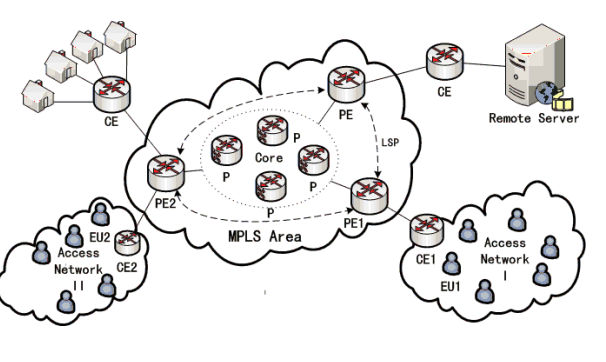
\includegraphics[width=0.67\linewidth]{Images/architecture-mpls}
	\end{center}
	\caption{Architecture du réseau mpls}
\end{figure} 


On trouve trois types différents de routeurs dans l'architecture de réseau MPLS : les routeurs PE et les routeurs P qui sont activés pour MPLS, et les routeurs CE qui sont des routeurs réguliers d'accès. Le routeur P est utilisé dans la zone centrale, son rôle principal est d’acheminer les paquets de données étiquetés tandis que le routeur PE est utilisé pour l'encapsulation et la désencapsulation des données ainsi que pour faire la liaison entre les routeurs P et CE.

Les routeurs PE fonctionnent avec deux types différents de routage : le premier protocole s’applique entre PE et CE pour modifier les informations d’adresse IP et de connexion tandis que le deuxième protocole s’applique au sein de la communication entre P et PE pour distribuer des étiquettes et gérer les LSP (chemins de distribution d’étiquettes).
 \subsubsection{Mécanisme de transfert de données dans une architecture de réseau MPLS de base  }
 La procédure de transfert de données entre deux utilisateurs dans deux réseaux d'accès différents est décrite comme suit,les paquets IP sont envoyés à CE, qui vérifie ensuite l'adresse de destination et recherche dans sa table de routage pour déterminer si les paquets de données doivent être transmis à un PE ou à d'autres utilisateurs dans le même réseau d'accès. 
 
 Ensuite, les paquets sont envoyés jusqu'au PE, qui vérifie à nouveau l'adresse de destination et choisit les étiquettes correspondantes à ajouter aux paquets en fonction de sa base de données FEC (Classe d'Équivalence de Transfert). La FEC assure le stockage de la relation de mappage entre les étiquettes sortantes et certaines adresses de destination.
  
  Après l'encapsulation, les paquets de données étiquetés sont envoyés aux routeurs P pour un acheminement rapide dans la zone centrale. Chaque saut pour un paquet de données dans la zone MPLS doit être accompagné d'un commutation d'étiquette. Après avoir suivi la route prédéfini et traversé la zone centrale, les paquets étiquetés arrivent au PE où ils sont désencapsulés et transférés à CE, qui vérifie ensuite l'adresse de destination et envoie le paquet de données à l'utilisateur.
  \subsection{VPN}
  \subsubsection{Définition }
  Un VPN est un réseau privé construit au sein d'une infrastructure de réseau public, telle que l'Internet. Il permet à des utilisateurs distants de se connecter de manière sécurisée en créant un tunnel crypté entre l'appareil de l'utilisateur et le réseau privé. Cette méthode assure la confidentialité et la sécurité des données échangées. Le VPN permet aux utilisateurs d'accéder aux ressources du réseau privé, telles que des fichiers, des applications et des imprimantes, comme s'ils étaient physiquement connectés au réseau local.      
  
  \subsubsection{les technologies VPN  }
  \begin{itemize}
  	\item[$\bullet$]\textbf{ IPSec :} 
  	
  	IPSec est appliqué au niveau de la couche réseau sans être en combinaison avec d'autres protocoles. Il fournit une collection de protocoles normalisés et de techniques pour établir des connexions VPN sécurisées. En assurant l’authentification, l’encapsulation et l’intégrité des paquets, IPSec garantit la sécurité des données. De plus, il peut établir des tunnels VPN entre des passerelles IPSec de différents fabricants grâce à sa normalisation. Bien que IPSec détermine les méthodes et les protocoles d'échange de base, il ne spécifie pas le niveau de sécurité à utiliser.
  	
  	Il existe deux modes de base de connexions IPSec. Dans le mode transport, un en-tête IPSec est ajouté à l'en-tête IP d'origine, contenant des informations d'authentification et d'intégrité. En revanche, dans le mode tunnel, chaque paquet IP d'origine est entouré d'un nouveau paquet IP comprenant un nouvel en-tête IP et l'en-tête IPSec. Ainsi, les informations sur le contenu du paquet IP d'origine sont cachées dans la charge utile du nouveau paquet IP.
  	
  	Lors de l'établissement d'une connexion IPSec, il y a deux phases de négociation. Pendant la première phase, la SA pour IKE est négociée, sans chiffrement ni authentification de données. Par contre, les deux partenaires doivent s'authentifier et échanger les clés en utilisant l'algorithme de chiffrement asymétrique à clé publique, Diffie-Hellman. Une fois les clés échangées, la phase deux est initiée. Pendant cette phase, déjà protégée, les paramètres des tunnels VPN sont négociés, y compris les clés de chiffrement symétriques, les informations d'expiration des clés, la politique de sécurité et les routes réseau. Après cela, les données peuvent être échangées de manière sécurisée.
  \end{itemize}
    \begin{itemize}
  	\item[$\bullet$]\textbf{L2TP :} 
  	
  	L2TP est le protocole de tunnelisation appliqué au niveau de la couche de liaison de données, il est basé sur le protocole de transfert L2F(Layer Two Forwarding), Il permet d'encapsuler une trame de la couche de liaison de données complète dans un paquet UDP au niveau de transport. Ce paquet UDP, transportant la trame de la couche deux, comprend plusieurs champs de données ,on trouve une en-tête UDP, des bits de contrôle représentant diverses options, la version et la longueur du paquet.
  	
  	 Ensuite, les champs de numéro de séquence et d'identifiant de tunnel qui permettent de suivre la connexion VPN actuelle pour assurer le traitement correct des paquets.
  	 
  	  Enfin, la trame de la couche deux qui contient des éléments tels que les adresses de contrôle d'accès au support (MAC) et la charge utile.
  	Pour garantir l'authentification et la confidentialité, l'encapsulation seule d'une trame de couche deux dans un paquet UDP n'est pas suffisante. C'est pourquoi le L2TP est souvent combiné avec IPSec en mode transport, en ajoutant l'en-tête IPSec devant l'en-tête L2TP. 
  \end{itemize}
     \begin{itemize}
  	\item[$\bullet$]\textbf{PPTP:} 
  	
  Le protocole de tunnelisation point-à-point de Microsoft est une extension du protocole point-à-point (PPP) et est pris en charge par toutes les versions de Microsoft Windows. 
  
  Pour établir une connexion VPN, PPTP utilise deux types différents de paquets , on trouve les paquets GRE (Generic Routing Encapsulation) qui transportent la charge utile du VPN en ajoutant l’en-tête GRE au paquet d’origine. L’en-tête GRE est assez similaire à l’en-tête L2TP et contient divers bits de contrôle, numéros de séquence et de tunnel. On trouve aussi les messages de contrôle PPTP, qui sont simplement des paquets TCP contenant des informations de contrôle telles que les demandes et réponses de connexion, les paramètres de connexion et les messages d'erreur.
  
  Microsoft utilise le protocole d'authentification par challenge (MS-CHAP) pour authentifier les deux partenaires de tunnel, car ni GRE ni les messages PPTP ne fournissent d'authentification ou de chiffrement.
 
  PPTP peut être utilisé pour établir des connexions VPN entre les réseaux des fournisseurs de services Internet et leurs clients, qui n'ont pas besoin d'installer de logiciel VPN supplémentaire. 
  \end{itemize}
  \subsection{les connexions dédiées}
  
  Les lignes dédiées ou spécialisées sont des connexions point à point ou multipoint qui permettent la transmission de données à des débits moyens et élevés. Ces connexions offrent une bande passante garantie et une faible latence, ce qui les rend idéales pour les applications qui nécessitent une communication rapide et fiable entre des sites distants.
 
  Les premiers liens numériques dédiés ont été développés dans les années 1970.  On parle du lien T1 comme un exemple , il utilise deux paires torsadées pour transmettre à des débits allant jusqu'à 1,544 Mbit/s dans les deux sens (avec 24 canaux vocaux). De manière similaire, le lien E1 offre une bande passante de 2,048 Mbit/s (avec 32 canaux vocaux). Ces types de connexions sont couramment utilisés pour relier des réseaux locaux (LAN) distants.
  
  Pour les connexions à longue distance, des câbles coaxiaux sont souvent utilisés, avec des répéteurs disposés tous les 60 kilomètres environ. Ces répéteurs sont nécessaires pour régénérer le signal et maintenir la qualité de la transmission sur de longues distances.
  En résumé, les lignes dédiées fournissent une connectivité haut débit et fiable entre des sites distants, ce qui en fait un choix privilégié pour les entreprises et les organisations qui ont besoin d'une communication stable et rapide entre leurs différentes implantations.
  \subsection{les réseaux Frame Relay}
  Le réseau Frame Relay est une technologie largement utilisée dans les années 1990 et au début des années 2000 pour connecter des sites distants via des connexions de réseau à commutation de paquets.
  
  Le principe du Frame Relay est de découper les données en petits paquets appelés "frames" et de les transmettre sur le réseau en utilisant des circuits virtuels. Ces circuits virtuels étaient établis entre les sites distants et étaient gérés par les équipements du fournisseur de services. Chaque paquet (ou frame) contient une étiquette d'identification qui permettait au réseau de router le paquet vers sa destination appropriée.
  
  Les réseaux Frame Relay offrent plusieurs avantages par rapport aux lignes dédiées traditionnelles. Tout d'abord, ils sont plus flexibles car ils permettent de partager une même liaison entre plusieurs sites distants . De plus, les circuits virtuels pouvaient être configurés et reconfigurés rapidement en fonction des besoins de l'entreprise, offrant ainsi une grande souplesse.
  \subsection{Les réseaux ATM }
  
  Les réseaux ATM (Asynchronous Transfer Mode) est une technologie largement déployée dans les années 1990 et au début des années 2000. Contrairement au Frame Relay, qui repose sur la commutation de paquets, l'ATM est basé sur la commutation de cellules. Chaque cellule ATM avait une taille fixe de 53 octets, ce qui assure un traitement plus efficace et prévisible du trafic.
  
  Les réseaux ATM sont utilisés pour transporter le trafic généré par une grande variété d'applications, chacune ayant des caractéristiques de trafic et des exigences de performances réseau différentes. 
  Pour répondre efficacement à cet environnement multi-applications, la couche ATM définissait un ensemble sophistiqué de fonctions et de procédures de gestion du trafic.
  Parmi les principaux objectifs de ces fonctions et procédures de gestion du trafic de la couche ATM, on peut citer :
  \begin{itemize}
  \item Protéger le réseau et les utilisateurs afin d'atteindre les objectifs de performance du réseau.
  \item Optimiser l'utilisation des ressources du réseau.
  \item Protéger les applications contre la congestion du réseau.
\end{itemize}
\section{Problématique}

Dans un monde où les entreprises évoluent rapidement, la nécessité d'une connectivité réseau agile et flexible est devenue indisponsable surtout dans le milieu militaire . 
Les solutions traditionnelles de mise en réseau peinent souvent à répondre aux exigences changeantes des entreprises, entraînant des inefficacités opérationnelles et des coûts élevés. 

Tout d'abord, les réseaux Frame Relay et ATM ont été critiqués pour leur manque de flexibilité et d’ Adaptabilité . la Configuration et la reconfiguration des circuits virtuels dans un réseau Frame Relay, par exemple, pouvait être Pénible et nécessite souvent l'intervention du fournisseur de services, ce qui entraîne des délais et des coûts supplémentaires.

De plus, ces technologies étaient souvent limitées en termes de bande passante et ne pouvaient pas toujours s'adapter efficacement aux besoins changeants des entreprises, en particulier avec l'émergence de nouvelles applications gourmandes en bande passante telles que la vidéoconférence et la VoIP.

Les connexions dédiées, bien qu'elles garantissent une bande passante stable et une faible latence, peuvent être coûteuses à mettre en place et à entretenir, notamment pour les déploiements multi-sites dans le domaine militaire. 
face aux défis posés par les infrastructures réseau traditionnelles, il est impératif de rechercher des solutions innovantes qui révolutionne la façon dont les entreprises gèrent leur infrastructure réseau ,une approche qui offre une connectivité robuste et évolutive tout en simplifiant la gestion globale du réseau.

Tout d'abord, on parle d’une connectivité multicloud, permettant aux entreprises de tirer parti de multiples fournisseurs de services cloud sans compromettre la performance ou la sécurité. Cette capacité à intégrer facilement des services cloud dans l'infrastructure réseau offre une flexibilité et une agilité exceptionnelles. elle permet aux entreprises de s'adapter rapidement aux changements du marché et aux nouvelles exigences métier.
De plus, une utilisation efficace des ressources réseau en tirant parti de la diversité des chemins de données disponibles, qu'il s'agisse de connexions Internet, de liaisons MPLS ou d'autres types de connexions. En équilibrant intelligemment le trafic sur ces différents chemins, on garantit une performance optimale et une disponibilité élevée, même dans des conditions de réseau variables. Cette capacité à optimiser la bande passante disponible est essentielle pour répondre aux besoins croissants en termes de volume de données et d'applications gourmandes en bande passante.

La sécurisation des communications réseau revêt aussi une importance majeure en offrant un chiffrement de bout en bout et des fonctionnalités avancées de pare-feu et de prévention des intrusions. En sécurisant les communications réseau à tous les niveaux, on garantit la confidentialité et l'intégrité des données, même lorsqu’on traverse des réseaux non sécurisés comme Internet. Cette sécurité renforcée est particulièrement importante dans un environnement où les cybermenaces sont de plus en plus sophistiquées et omniprésentes.

Enfin, la simplification de la gestion globale du réseau en offrant une interface centralisée et intuitive pour la configuration, la surveillance et le dépannage. En consolidant les opérations réseau dans une seule plateforme, on  réduit la complexité et les coûts associés à la gestion de multiples appareils et systèmes.Cette simplification de la gestion est essentielle pour décharger les équipes informatiques des tâches fatigantes, leur permettant ainsi de se concentrer pleinement sur des initiatives stratégiques à forte valeur ajoutée.
\section{Solution proposé }

Face à la nécessité croissante d'une infrastructure réseau agile et flexible, les solutions traditionnelles rencontrent souvent des difficultés pour s'adapter aux exigences évolutives et complexes.C'est dans ce contexte que les technologies de Software-Defined Networking (SDN) émerge comme l’un des solutions innovantes , offrant des perspectives nouvelles pour la gestion et l'optimisation des réseaux d'entreprise.

\subsection{Généralité sur SDN }

Le réseau défini par logiciel (SDN ) est une approche innovante pour concevoir, mettre en œuvre et gérer des réseaux qui séparent le contrôle du réseau (plan de contrôle) et le processus de transfert de données (plan de données) pour une meilleure expérience utilisateur.
SDN facilite le déploiement d'applications au sein des organisations et permet une livraison flexible . De plus il offre la capacité de mettre à l'échelle les ressources réseau en parallèle avec les besoins des applications et des données, et réduisant à la fois les dépenses en capital (CapEX) et les dépenses opérationnelles (OpEX). 
\subsection{Architecture du SDN   }
L'architecture du SDN (Software-Defined Networking) est divisée verticalement en trois couches comme montre la figure.

\begin{figure} [H]
	  \hspace{0.9cm}
	\begin{center}
        \centering
		\hspace*{-0.5cm}
		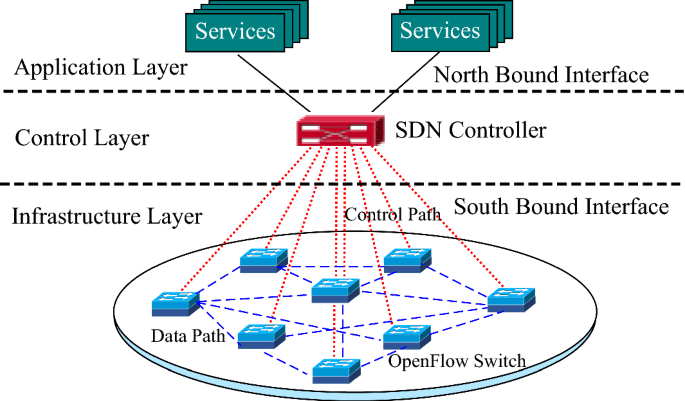
\includegraphics[width=0.67\linewidth]{Images/SDN-arch}
	\end{center}
	\caption{Architecture du SDN}
\end{figure} 
\subsubsection{Couche d'infrastructure }

C'est la couche inférieure qui comprend les commutateurs, les routeurs et d'autres périphériques réseau physiques. Ces périphériques, appelés des éléments de commutation, sont chargés de transférer les paquets et sont responsables de l'acheminement réel du trafic en fonction des instructions fournies par la couche de contrôle.

Dans le contexte du SDN, la séparation entre le contrôle et le plan de données exige que le plan de données soit accessible à distance pour un contrôle basé sur un logiciel via une interface Sud (Southbound interface) ouverte et indépendante du fournisseur.
\subsubsection{Couche de contrôle }

Cette couche est responsable de la logique de contrôle du réseau et est considérée comme l'entité fondamentale dans l'architecture SDN. Elle comprend un contrôleur logiciel centralisé chargé de gérer les communications entre les applications réseau et les appareils via des interfaces ouvertes.

La couche de contrôle SDN est souvent appelée le système d'exploitation réseau (NOS) car elle prend en charge la logique de contrôle du réseau et fournit à la couche d'application une vue abstraite du réseau global, contenant suffisamment d'informations pour spécifier des politiques tout en masquant tous les détails de mise en œuvre.

Dans une configuration de contrôle SDN distribué, des APIs Est-Ouest sont nécessaires pour permettre à plusieurs contrôleurs SDN de communiquer entre eux et d'échanger des informations réseau. 

\subsubsection{Couche d'application }

C'est la couche supérieure où résident les applications et les services réseau qui sont des programmes de contrôle conçus pour mettre en œuvre la logique et les stratégies de contrôle du réseau. Cette couche de niveau supérieur interagit avec la couche de contrôle via une API Nord ouverte.Ainsi, les applications SDN communiquent leurs besoins réseau au contrôleur SDN qui les traduit en commandes spécifiques au Sud et en règles de transfert dictant le comportement des périphériques de plan de données individuels.

Le routage, l'ingénierie du trafic (TE), les pare-feu et l'équilibrage de charge sont des exemples d'applications SDN courantes s'exécutant sur les plates-formes de contrôle existantes . 
\subsection{la solution SD-wan  }
aprés avoir explorer en profondeur l'architecture et les fonctionnalités du SDN, il est important de souligner que le SD-WAN(Software-Defined Wide Area Network), émerge comme une évolution naturelle de cette technologie révolutionnaire.

Le SD-WAN tire parti des fondements du SDN en séparant le plan de contrôle du plan de données, permettant ainsi une gestion centralisée et une adaptation dynamique du trafic sur des réseaux étendus. En intégrant des fonctionnalités avancées telles que le routage intelligent, la gestion dynamique des liens, et la qualité de service (QoS) basée sur les applications, le SD-WAN offre une agilité et une flexibilité accrues pour répondre aux besoins changeants des entreprises en matière de connectivité réseau.

\section*{Conclusion }

Dans ce premier chappitre ,nous avons examiné attentivement l'étude de l'existant, identifié la problématique associée et présenté une première approche de solution. Dans le chapitre suivant, nous passerons à une analyse plus détaillée et à une spécification approfondie des besoins, afin de mieux comprendre les exigences spécifiques et les objectifs à atteindre dans le cadre de notre projet.
		%
	\chapter{Analyse et spécification des besoins }
	\newpage
\section*{Introduction }

Ce chapitre se concentre sur l'analyse et la spécification des besoins, en distinguant entre les besoins fonctionnels et non fonctionnels. Nous procéderons ensuite à une étude comparative des solutions SD-WAN pour choisir la plus adaptée.

\section{Les besoins fonctionnels et non fonctionnels  }
\subsection{Les besoins fonctionnels }
\subsubsection{Routage intelligent  }

Le routage intelligent représente la capacité d'un système à diriger le trafic de manière dynamique et efficace en fonction des exigences de performance et des politiques définies. Dans le contexte des réseaux SD-WAN, plusieurs protocoles de routage sont utilisés. Parmi eux, le BGP (Border Gateway Protocol) est un protocole de routage largement utilisé pour échanger des informations de routage entre différents systèmes autonomes (AS) sur Internet. Dans un environnement SD-WAN, le BGP facilite l'échange de routes entre les sites distants et le centre de données centralisé, assurant ainsi une connectivité fiable et dynamique.

De plus, l'OSPF (Open Shortest Path First) est un protocole de routage intérieur beaucoup utilisé dans les réseaux d'entreprise pour calculer les chemins les plus courts entre les routeurs. Dans un déploiement SD-WAN, l'OSPF peut être utilisé pour optimiser la connectivité entre les différents sites distants et les nœuds du réseau SD-WAN.

\subsubsection{Optimisation du trafic  }
Il y’avait de nombreuses solutions qui  ont été proposées pour transporter plus de trafic et soutenir un partage équitable, l’idée la plus importante est de définir des priorités pour différents types de trafic.
Dans SDWAN, le trafic est classé en trois catégories , on parle du trafic interactif, élastique et de fond, en fonction des caractéristiques des services qui les génèrent.  Prenons l’exemple des requêtes et des réponses dans les moteurs de recherche, ils sont considérées comme du trafic interactif puisque il sont très sensibles à la perte de paquets et aux retards, et elles devraient être planifiées avec la plus haute priorité .

SDWAN permet au trafic interactif de préempter la bande passante. Il est envoyé dès que possible, alors que, pour les autres types de trafic, tels que le trafic élastique et de fond, SDWAN calcule la quantité de trafic que chaque service peut envoyer et configure le plan de données du réseau pour transporter ce trafic tout en tenant compte de l'équité entre services similaires. 

Par cet méthode , SDWAN peut optimiser la bande passante et  prioriser les applications critiques pour garantir une expérience utilisateur optimale.

\subsubsection{Gestion centralisée  }

La gestion centralisée dans un réseau SD-WAN offre aux administrateurs la possibilité de contrôler tous les aspects du réseau à partir d'une seule interface centralisée. Cela inclut la configuration des appareils, la définition des politiques de sécurité, la surveillance des performances du réseau, la gestion de la bande passante, et bien plus encore. 

Grâce à cette approche centralisée, les administrateurs peuvent effectuer des tâches de gestion de manière efficace et cohérente sur l'ensemble du réseau, ce qui simplifie les opérations et garantit une visibilité globale sur l'état du réseau.
\subsubsection{Sécurité avancée   }

La sécurité avancée dans SD-WAN implique l'intégration de plusieurs fonctionnalités de sécurité pour protéger le trafic réseau contre les menaces potentielles. Cela inclut le chiffrement des données qui est un élément  essentiel pour garantir la confidentialité des informations transitant à travers le réseau SD-WAN. Les pare-feu intégrés filtrent et contrôlent le trafic en fonction de règles prédéfinies, bloquant les communications non autorisées et détectant les tentatives d'intrusion.

De plus, les IDS/IPS assurent la détection des menaces en utilisant des technologies avancées telles que l'apprentissage automatique et l'analyse comportementale pour identifier les activités malveillantes ou suspectes sur le réseau, y compris la détection des logiciels malveillants et des attaques par déni de service distribué (DDoS).

Enfin, l'intégration d'un SIG, qui est une passerelle Internet sécurisée, permet de centraliser et de consolider les fonctions de sécurité au niveau de la connectivité Internet. Cela permet de filtrer le trafic Internet avant qu'il n'atteigne les sites distants, réduisant ainsi la surface d'attaque et améliorant la sécurité globale du réseau. 
\subsubsection{La segmentation }

La segmentation réseau divise un réseau en plusieurs segments ou sous-réseaux,comme montre la figure . Elle permet d'améliorer la surveillance et le contrôle du réseau grâce à des politiques. Elle offre aussi la possibilité d'améliorer les aspects de sécurité , en empêchant l'accès simultané à l'ensemble des ressources. Par conséquent, en cas d'intrusion, seule la partie des ressources exposée à l'attaque sera compromise, alors que le reste des ressources restera sécurisé.
\begin{figure} [H]
	
	\begin{center}
		\centering
		\hspace*{-0.5cm}
		
	\end{center}
	\caption{La ségmentation dans SD-WAN }
\end{figure} 
\subsubsection{Haute disponibilité  }

Parmi les mécanismes de redondance et de basculement pour garantir la disponibilité continue des services, même en cas de panne de lien ou de périphérique dans le réseau, on trouve la redondance des liens, qui implique la mise en place de plusieurs connexions réseau pour un même point d'accès. 


De plus, la redondance des périphériques consiste à disposer de plusieurs équipements réseau configurés pour prendre le relais en cas de défaillance d'un périphérique principal. 
Les protocoles de basculement automatique, tels que HSRP, VRRP ou FHRP, permettent une transition transparente vers les équipements de secours en cas de défaillance.


Le load balancing peut aussi être utilisé pour répartir le trafic entre plusieurs équipements ou liens réseau redondants, améliorant ainsi les performances de l'application en optimisant l'agrégation, l'accélération et le déchargement. 

Ainsi, en cas de défaillance d'un équipement ou d'un lien, le trafic peut être automatiquement redirigé vers d'autres ressources disponibles, assurant ainsi la continuité du service sans interruption pour les utilisateurs finaux.

\subsubsection{Évolutivité }

la gestion centralisée facilite l'extension du réseau SD-WAN en permettant l'ajout de nouveaux sites et appareils de manière transparente. Les administrateurs peuvent facilement provisionner de nouveaux équipements, mettre à jour des configurations et adapter le réseau aux besoins changeants de l'entreprise, le tout à partir d'une interface centralisée.

\subsection{Les besoins non fonctionnels }
\subsubsection{Performance   }

SD-WAN est capable de fournir des performances optimales en termes de débit, Garantir des temps de réponse rapides et une faible latence pour les applications critiques afin de garantir une expérience utilisateur satisfaisante pour les applications et les services hébergés sur le réseau.
Fiabilité : Assurer une disponibilité élevée du réseau et des applications, avec des mécanismes de redondance et de récupération en cas de défaillance.


\subsubsection{Coût  }

Le SD-WAN offre une rentabilité accrue en minimisant les dépenses liées à l'exploitation et à la maintenance, tout en améliorant l'efficacité opérationnelle.

Contrairement aux technologies traditionnelles qui exigent souvent des déplacements sur site pour l'installation de nouvelles configurations et mises à jour, le SD-WAN permet des déploiements à distance, réduisant ainsi les coûts associés à la main-d'œuvre et aux déplacements.

\subsubsection{Interopérabilité  }

Le SD-WAN est compatible avec les infrastructures et les systèmes existants de l'entreprise .Cette compatibilité permet une intégration harmonieuse du SD-WAN avec les équipements réseau existants, tels que les routeurs, les commutateurs et les pare-feu, ainsi qu'avec les applications et les services cloud utilisés par l'entreprise et c’est grâce a cette interopérabilité, les entreprises peuvent bénéficier des avantages du SD-WAN tout en minimisant les perturbations et les coûts associés à la transition vers cette technologie.

\section{Étude comparative et choix de la solution SD-WAN   }
\subsection{Étude comparative  }
%\begin{tabular}{|p{2.5cm}|p{2.5cm}|p{2.5cm}|p{2.5cm}|p{2.5cm}|}
\begin{table}[H]
	\begin{center}
		\caption{Tableau comparatif  }
		
		\hspace*{-0.5 cm}	\begin{tabular}{|p{3cm}|p{3cm}|p{3cm}|p{3cm}|p{3cm}|}
			\hline
			\centering
			& Cisco & Fortinet & Silver Peak & Versa\\
			\hline
			\centering
			
			La plateforme prend en charge à la fois le routage classique et le SD-WAN. & -Services de routage classiques complets.
			- Migration fluide et intégration harmonieuse des fonctionnalités SD-WAN avec le routage classique sur une même plateforme.
			& -Le déploiement d'un SD-WAN n'implique ni l'ajout de composants supplémentaires ni la nécessité de modifier votre infrastructure existante. & -Migration sans protection des investissements.
			
			-fonctionnalités classiques de routage restreintes sur la même plateforme SD-WAN.
			& - L'utilisation d'un SD-WAN nécessite l'ajout de matériel. \\
			
			\hline
			
			
			\centering
			Architecture SD-WAN personnalisée& - Les composants dédiés à l'évolutivité et aux performances, répartis entre les plans de contrôle, de données et de gestion, fournissent une architecture compatible avec SDN.
			-Flexibilité pour ajuster l'architecture à l'objectif de l'entreprise.
			- le déploiement dans le cloud est pris en charge et géré par l'équipe Cisco Cloud Ops.
			&- Ancienne infrastructure reposant sur un pare-feu.&- Ancienne infrastructure combinant les plans de contrôle et de données.&- Des composants spécialisés pour le contrôle, les données et la gestion.
			\\
			\hline
		\end{tabular}
	\end{center}
\end{table}	
\begin{table}[H]
	\begin{center}
		
		\hspace*{-0.5 cm}	\begin{tabular}{|p{3cm}|p{3cm}|p{3cm}|p{3cm}|p{3cm}|}
			\hline
			\centering
			\centering
			Modèle de politique évolutif & -La sélection dynamique des chemins permet aux applications critiques d'éviter automatiquement les problèmes de réseau.
			- la microsegmentation et la gestion des politiques basée sur l'identité facilitent l'application cohérente de politiques multisites pour assurer une expérience utilisateur uniforme.& - La gestion séparée des politiques pour le SD-WAN et le pare-feu complique l'ingénierie du trafic et la transmission de politiques centralisées pour les plans de contrôle et de données.& -Bien que les politiques puissent être créées et réutilisées pour répondre aux besoins de l'entreprise, la microsegmentation et l'application de politiques multidomaines sont restreintes.& Bien qu'il soit possible d'effectuer l'ingénierie du trafic en fonction de politiques sensibles aux applications, l'application de politiques multidomaines est restreinte.
			\\
			\hline
			
			
			\centering
			AAAAAAA &BBBBBBB\\
			\hline
			\centering
			
			5) Nez en l’air &   6) Sur le dos \\
			\hline
		\end{tabular}
	\end{center}
\end{table}	


\subsection{Choix de la solution SD-WAN  }
Le choix de la solution dépend de quatre éléments essentiels ,l'infrastructure réseau, la sécurité réseau, l'intégration cloud et la périphérie du réseau.
\subsubsection{L'infrastructure réseau }

La plateforme Cisco offre une solution complète en prenant en charge à la fois le routage classique et le SD-WAN, offrant ainsi une flexibilité et une évolutivité optimales pour les entreprises. Elle propose des services de routage classiques complets, ce qui garantit une transition fluide et une intégration harmonieuse des fonctionnalités SD-WAN avec le routage traditionnel sur une même plateforme. 

De plus, le déploiement d'un SD-WAN avec Cisco n'implique ni l'ajout de composants supplémentaires ni la nécessité de modifier l’infrastructure existante, ce qui réduit les coûts et simplifie le processus. Par contre, d'autres solutions comme Fortinet, Silver Peak et Versa peuvent présenter des limitations telles que des fonctionnalités de routage restreintes sur la même plateforme SD-WAN ou la nécessité d'ajouter du matériel pour utiliser le SD-WAN, ce qui peut rendre la migration moins fluide et moins rentable. Ainsi, la simplicité et l'intégration transparente font de Cisco une option supérieure pour les entreprises cherchant à adopter le SD-WAN.

La force de Cisco réside dans sa capacité à offrir une architecture SD-WAN personnalisée. Avec des composants dédiés à l'évolutivité et aux performances répartis entre les plans de contrôle, de données et de gestion, Cisco assure une compatibilité avec les principes du SDN. Cette approche permet d'ajuster facilement l'architecture en fonction des objectifs de l'entreprise. De plus, Cisco propose une prise en charge complète du déploiement dans le cloud, avec une gestion assurée par l'équipe experte de Cisco Cloud Ops. Comparé avec  d'autres solutions  qui repose sur des infrastructures Anciennes reposant sur un pare-feu et combinant les plans de contrôle et de données..cette approche garantit une efficacité opérationnelle et une meilleure adaptabilité aux besoins changeants des entreprises.

En outre,cisco se distingue par son modèle de politique évolutif, qui offre une sélection dynamique des chemins pour permettre aux applications critiques d'éviter automatiquement les problèmes de réseau. De plus, sa microsegmentation et sa gestion des politiques basée sur l'identité facilitent une application cohérente des politiques multisites, garantissant ainsi une expérience utilisateur uniforme.Contrairement à certaines autres solutions, la gestion distincte des politiques pour le SD-WAN et le pare-feu ajoute une complexité à l'ingénierie du trafic et à la transmission des politiques centralisées pour les plans de contrôle et de données. De même pour d’autres solutions, bien que les politiques puissent être créées et réutilisées pour répondre aux besoins de l'entreprise, les capacités de microsegmentation et de gestion des politiques multidomaines sont limitées dans d'autres solutions.

En résumé, Cisco reste  un choix supérieur en offrant une architecture SD-WAN personnalisée et une solution complète prenant en charge à la fois le routage classique et le SD-WAN , garantissant ainsi une évolutivité et une flexibilité optimales pour répondre aux besoins variés des entreprises.
\subsubsection{la sécurité réseau }

Cisco intègre la technologie "Silicon root of trust" dans son matériel pour une sécurité renforcée au niveau du  matériel, offrant ainsi une protection intégrée contre les attaques visant les bases du réseau et les accès non autorisés. En revanche, d'autres solutions telles que Fortinet, Silver Peak et Versa présentent des faiblesses en matière de sécurité. En effet, l'absence de détails concernant la protection intégrée offerte par leurs circuits intégrés personnalisés expose les entreprises à des risques de sécurité plus élevés. De plus, bien que ces solutions fournissent un matériel professionnel standard, elles ne disposent pas d'une solution de protection fiable connue, ce qui augmente le potentiel d'attaques ou d'accès non autorisés.

La segmentation réseau est une approche importante de l'architecture SD-WAN, et Cisco offre une segmentation MPLS/VRF complète et éprouvée. Cette solution prend en charge les topologies multisegments et la mutualisation, ce qui permet aux entreprises d'optimiser l'utilisation de leur infrastructure réseau tout en assurant la sécurité et la performance des données. En revanche, des solutions telles que Fortinet présentent des capacités de segmentation restreintes, avec des configurations VDOM complexes qui limitent la flexibilité pour créer des topologies multisegments dynamiques et adaptables aux besoins évolutifs des entreprises. De même, Silver Peak propose une segmentation basée sur VRF, mais elle est limitée en termes de routage avec le protocole OSPF et de priorisation des pairs.

En outre ,l'analyse du trafic chiffré est essentielle pour détecter les menaces potentielles et assurer la sécurité du réseau. Cisco a la capacité d’identifier les logiciels malveillants en comparant les modèles SHA chiffrés, sans avoir besoin de les déchiffrer, offrant ainsi une protection efficace contre les attaques. En revanche, des solutions comme Fortinet présentent une faiblesse en termes de robustesse de leur solution d'analyse du trafic chiffré, qui peut ne pas être suffisamment efficace pour sécuriser les infrastructures ou les périphériques réseau. De même, Silver Peak ne permet pas la détection des malwares chiffrés, ce qui expose les entreprises à des risques de sécurité plus élevés. 

En résumé, Cisco est le choix optimal pour la sécurité réseau, il propose la  technologie "Silicon root of trust" offrant une sécurité intégrée au niveau matériel, une segmentation MPLS/VRF complète, et une capacité à détecter les logiciels malveillants sans déchiffrement. En comparaison avec des solutions comme Fortinet et Silver Peak, ils  présentent des lacunes en matière de sécurité intégrée et de segmentation réseau, ce qui expose les entreprises à des risques de sécurité accrus.

\subsubsection{L'intégration cloud  }

Pour la connectivité multicloud,Cisco est le meilleur choix grâce à son processus automatisé de déploiement sur diverses plateformes cloud telles qu'Amazon Web Services (AWS), Microsoft Azure et Google Cloud Platform (GCP). Avec des instructions détaillées guidant chaque étape du déploiement, Cisco offre une connectivité multicloud efficace et facile à mettre en œuvre. 

En comparaison, des solutions telles que Fortinet présentent des workflows limités pour la connectivité multicloud, tandis que Silver Peak et Versa nécessitent une configuration manuelle pour le déploiement sur différents fournisseurs de cloud, ce qui compromet la rapidité et l'efficacité du déploiement.
\subsubsection{la périphérie du réseau  }

Cisco est le choix optimal en termes de stockage en offrant une automatisation IoT/OT avec des fonctionnalités de stockage et de calcul intégrées pour les sites distants, le tout pris en charge par la gamme de commutateurs Cisco Catalyst 8200. En revanche, des solutions telles que Fortinet, Silver Peak et Versa présentent des lacunes en termes de capacités d'hébergement de fonctions réseau virtuelles (VNF) en périphérie du réseau, avec une capacité limitée chez Versa, bien que ce dernier permet le déploiement de VNF sur les appliances Versa SD-WAN Edge.
En outre , Cisco offre  une intégration VoIP native grâce à ses plateformes Cisco Catalyst 8000 Edge, qui fournissent des services VoIP complets dans le cadre du SD-WAN et pour les piles de fonctions logicielles classiques IOS XE. De plus, Cisco est le seul fournisseur de SD-WAN à intégrer directement une adresse IP analogique/numérique dans un équipement terminal client unique, offrant ainsi une solution complète et native pour les besoins de voix sur IP. En comparaison, des solutions comme Fortinet souffrent d'une absence de fonctionnalité d'hébergement d'applications en périphérie du réseau, tandis que Silver Peak et Versa ne proposent aucune intégration native de la voix, ce qui peut limiter les fonctionnalités et l'efficacité des déploiements de communications unifiées.

\section*{Conclusion }

Dans ce chapitre, nous avons examiné en détail les besoins de notre infrastructure réseau, en mettant en évidence les critères fonctionnels et non fonctionnels essentiels. Après avoir comparé les différentes solutions SD-WAN disponibles, nous avons choisi la solution optimale. Dans le chapitre suivant, nous allons analyser et concevoir la solution SD-WAN pour répondre à nos besoins spécifiques.





		\chapter{Analyse et conception de la solution SD-WAN }



\section*{Introduction }
Ce chapitre présente l'analyse et la conception de la solution SD-WAN, en mettant l'accent sur le Cisco Viptela SD-WAN. Nous commencerons par une présentation générale de cette technologie avant d'examiner son architecture, ses fonctionnalités et ses composantes principales.

\section{Présentation du Cisco Viptela SD-WAN }
\subsection{Définition du  SDWAN }

Les réseaux SD-WAN (Software-Defined Wide Area Network) sont considérés comme une technologie révolutionnaire pour l'utilisation des services WAN. 

Le SD-WAN introduit le concept de "réseau piloté par les applications",c’est-à-dire le réseau n'est plus statique, mais il s'adapte en temps réel aux exigences des applications et des services utilisés. Sdwan propose une gestion centralisée et flexible et permet d'optimiser l'utilisation des ressources et de garantir une meilleure qualité de service.

Le SD-WAN a un impact majeur sur les services de communication convergente (CC) et les environnements WAN. Il incite à repenser l'utilisation des services réseau et ouvre la voie à de nouvelles possibilités pour la communication du futur.
\subsection{Histoire de Cisco Viptela et son intégration dans l'écosystème Cisco }

Cisco SD-WAN Viptela est issu de l'acquisition de la société Viptela par Cisco en 2017 viptela était reconnue pour sa méthode innovante en matière de SD-WAN en offrant une gestion centralisée et une connectivité sécurisée pour les entreprises distribuées. Son acquisition par Cisco a renforcé l'offre de SD-WAN de l'entreprise et permet une intégration harmonieuse dans l'écosystème Cisco , offrant aussi aux clients une solution SD-WAN complète et performante.
\subsection{Les avantages du cisco viptela SDWAN }

Viptela offre une variété  d'avantages pour les entreprises avec sa capacité à prendre en charge une infrastructure privée en nuage ou sur site, Viptela répond aux besoins de différentes configurations d'infrastructure selon les préférences et les exigences de l'entreprise. 

En offrant une connectivité flexible via des connexions Ethernet, LTE, T1 et DSL, Viptela permet aux entreprises de s'adapter à diverses conditions de connectivité tout en maintenant des performances optimales. Sa prise en charge des topologies WAN complexes avec un haut degré de personnalisation offre une grande souplesse dans la conception et la gestion des réseaux, adaptée aux besoins spécifiques de chaque entreprise.De plus, Viptela fournit une segmentation sécurisée de bout en bout, une gestion des menaces efficace et un contrôle automatisé des chemins, offrant ainsi une tranquillité d'esprit en matière de sécurité et de performances réseau. Son support pour l'intégration de multiples charges de travail virtuelles dans des environnements de cloud privé virtuel (VPC) permet une gestion centralisée et une optimisation des ressources.Bien que le coût par mégabit puisse être légèrement plus élevé en raison de ses fonctionnalités avancées telles que le routage avancé, le chaînage de services et la sécurité cloud, Viptela offre une valeur ajoutée significative en termes de flexibilité, de sécurité et de performances.

En utilisant des équipements tels que les routeurs intégrés ISR 4K ou les vEdge, Viptela garantit une intégration transparente dans l'infrastructure existante, facilitant ainsi la transition vers une solution SD-WAN sophistiquée et évolutive.

\section{Architecture du Cisco Viptela SD-WAN }
\subsection{Architecture logique  }
l'architecture d'un réseau étendu défini par logiciel (SD-WAN) se compose de trois couches superposées de bas en haut comprenant la couche de données, la couche de contrôle et la couche applicative comme montre la figure.
\begin{figure} [H]
	\begin{center}
		\centering
		\hspace*{-0.5cm}
		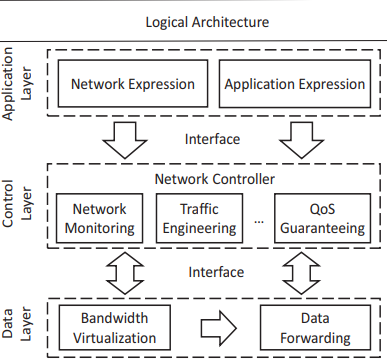
\includegraphics{../image/arch log}
	\end{center}
	\caption{Architecture-logique}
\end{figure} 
\subsubsection{    la couche de données }

Elle assure la virtualisation de bande passante et le transfert de données. la virtualisation de bande passante permet de maximiser l'utilisation des ressources de bande passante en combinant les différents  liens réseau couvrant un même emplacement pour former un pool de ressources partagées, ce qui améliore la performance globale du réseau et permet de répondre de manière plus efficace aux besoins de connectivité des utilisateurs et des applications.

Quant au transfert de données, il est réalisé par un d'éléments de réseau dédié pour le  transfert, principalement des commutateurs, utilisant la capacité de bande passante fournie par la virtualisation de bande passante pour acheminer les paquets de données de manière efficace à travers le réseau . Les deux éléments reçoivent des instructions du contrôleur de réseau situé dans la couche supérieure en utilisant des protocoles d'interface tels que OpenFlow. 
\subsubsection{ la couche de controle}
il existe plusieurs fonctions réseau ,dans la couche de contrôle ,  implémentées et gérées de manière indépendante. La séparation de ces fonctions permet aux opérateurs réseau de développer, de modifier, de déboguer et de supprimer l'une d'entre elles à faible coût sans affecter les autres . ansi les fonctions réseau peuvent être connéctées ,pour offrir une multitude de services et augmenter la flexibilité du réseau étendu défini par logiciel. Prenant par exemple la vue globale fournit par la surveillance du réseau pour l'ingénierie du trafic pour qu’elle puisse calculer une solution d'ordonnancement optimale à exécuter dans le réseau ,aussi La garantie de la qualité de service se charge de satisfaire les exigences des applications pendant la transmission des données. 

\subsubsection{  la couche d’application }
Avec l'émergence croissante d'applications ayant des exigences multiples et parfois contradictoires, il devient essentiel d'adapter les politiques réseau en tenant compte des spécificités de chaque application.
La couche d’application permet aux fournisseurs de réseau et aux développeurs d'applications de participer davantage au contrôle du réseau et de définir leurs exigences spécifiques et de haut niveau pour le réseau à travers l'expression réseau et l'expression d'application. Ces expressions sont capables de traduire ces exigences presque dans un langage naturel en configurations réseau conformes. 
\subsection{Architecture physique }

Dans la couche de données, se trouve un ensemble de commutateurs interconnectés par des liaisons physiques, formant ainsi une infrastructure réseau. Ces commutateurs sont contrôlés par un dispositif central appelé contrôleur réseau. Ce contrôleur peut être un serveur dédié ou un cluster de serveurs, selon la taille et la complexité du réseau. Au-dessus du contrôleur réseau, résident les applications spécifiques qui exploitent les fonctionnalités du réseau.
Les développeurs d'applications ainsi que les fournisseurs de réseau ont la possibilité d'exprimer leurs besoins et leurs exigences au contrôleur réseau. Celui-ci agit comme une interface entre les demandes des utilisateurs et les fonctionnalités du réseau sous-jacent. En fonction des spécifications reçues, le contrôleur réseau traduit ces demandes en politiques et configurations réseau appropriées,afin d'optimiser les performances du réseau et de répondre aux besoins des utilisateurs et des applications de manière efficace. 
\begin{figure} [H]
	\begin{center}
		\centering
		\hspace*{-0.5cm}
		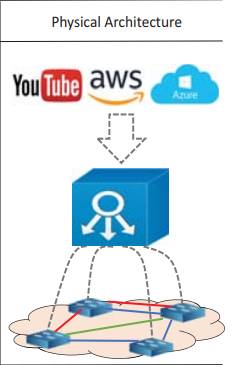
\includegraphics[height=6cm]{../image/arch phy}
	\end{center}
	\caption{Architecture-physique}
\end{figure} 

\section{Les fonctionnalités du Cisco Viptela SD-WAN }

Le Cisco Viptela SD-WAN offre  plusieurs fonctionnalités pour répondre aux besoins de connectivité réseau .
\subsection{Gestion centralisée  }

A travers vManage,on peut assurer l’administration centralisé du système, vManage représente le point principal de surveillance, d'inspection et de configuration de l'infrastructure du réseau. Des options diverses, comme montre la figure , sont mises à disposition grâce à elle.
\begin{figure} [H]
	\begin{center}
		\centering
		\hspace*{-0.5cm}
		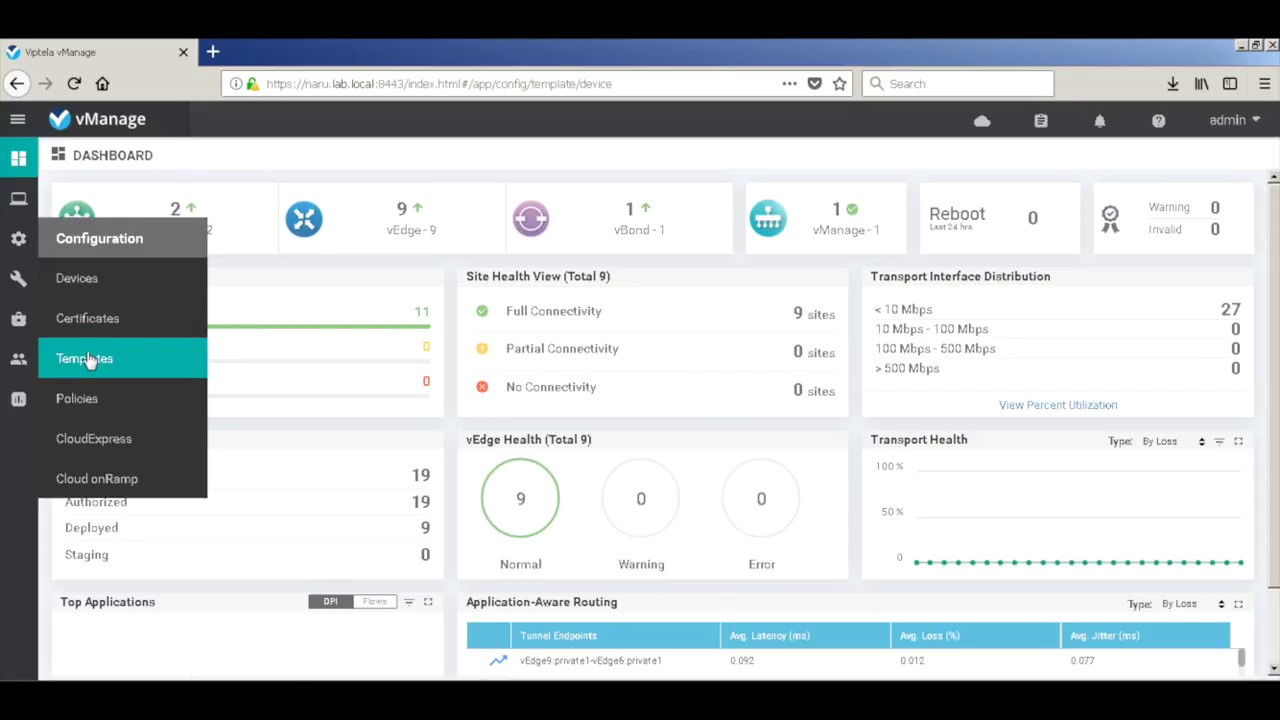
\includegraphics[height=7cm,width=10cm]{../image/Vmanage}
	\end{center}
	\caption{Interface vManage}
\end{figure} 
\subsubsection{Zero-touch provisioning (ZTP)   }
\begin{itemize}
	\item[$\bullet$]\textbf{  Principe :} 
	
	ZTP permet de configurer automatiquement de nouveaux équipements réseau sans intervention manuelle sur le périphérique lui-même, ce qui  simplifie et accélère le processus de déploiement.
\end{itemize}
\begin{itemize}
	\item[$\bullet$]\textbf{Mécanisme :} 
	
	Au début, le vEdge ou le cEdge reçoit l'adresse IP de l'ISP (Internet Service Provider). Dès qu'il est connecté au fournisseur de services, cela est réalisé grâce à DHCP (Dynamic Host Configuration Protocol), qui est configuré du côté du fournisseur de services. Par la suite, le Edge possède une URL ZTP prédéfinie et il peut maintenant atteindre le serveur DNS Viptela. En utilisant l'URL ZTP, le vEdge établit une connexion avec le serveur ZTP, où il vérifie son numéro de série, puis il est redirigé vers l'orchestrateur vBond qui vérifie lui-même le numéro de série et le certificat. Une connexion sécurisée est donc établie entre le Edge et vBond, formant ainsi le plan de contrôle du réseau. Une fois l'authentification du Edge effectuée, vBond envoie l'adresse IP de vManage et vSmart à l'Edge, et informe les autres contrôleurs de ce nouveau périphérique. Après avoir assuré son authenticité, vManage envoie une configuration prédéfinie vers le Edge, qui reçoit aussi la politique par vSmart. De cette façon, le Edge est correctement intégré au SD-WAN overlay et est prêt à échanger des messages OMP.
	
\begin{figure} [H]
	\begin{center}
		\centering
		\hspace*{-0.5cm}
		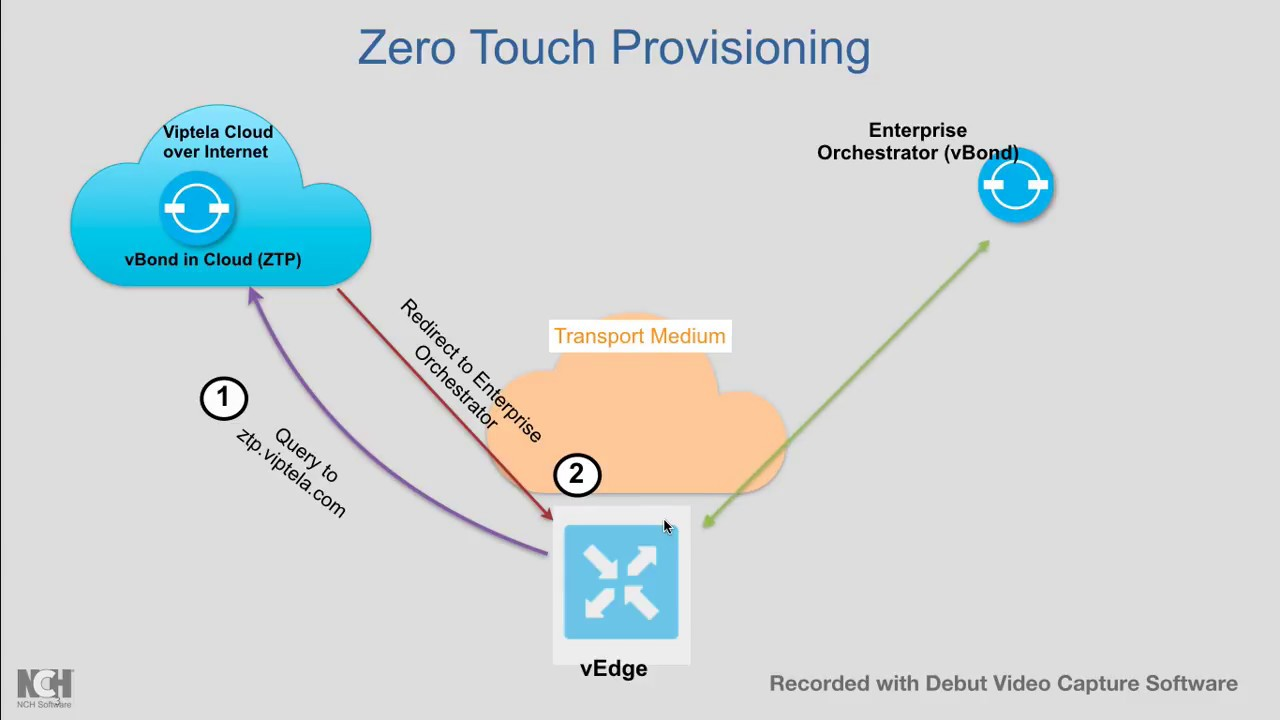
\includegraphics[height=7cm,width=10cm]{image/zttp}
	\end{center}
	\caption{Zero Touch Provisioning}
\end{figure} 
\end{itemize}
\subsubsection{Visibilité des applications  }

La visibilité des applications dans SD-WAN permet au client de voir à travers toute l'infrastructure jusqu'au niveau des flux des applications spécifiques.le client peut observer et comprendre le trafic réseau généré par différentes applications utilisées dans son environnement. 

Cette visibilité offre plusieurs avantages dans  l’identification rapide  de la source du problème, en examinant les flux d'application correspondants.

\subsubsection{Gestion des alertes et des notifications   }

les administrateurs peuvent obtenir des rapports de problème de bout en bout sans traçage.

Lorsqu'un problème critique est détecté  ou une situations qui nécessite  une intervention immédiate, sdwan génère automatiquement des alertes ou des notifications pour que les administrateurs peuvent être informés en temps réel.

\subsubsection{Rapidité d’exécution et Fiabilité Renforcée  }
Dans les réseaux traditionnels,la configuration est assurer via le cli , on se connecte au peripherique via TELNET/SSH ou CONSOLE et on peut modifier la configuration par la suite mais cela nécessite beaucoup de temps pour apporter des modifications massives à la configuration de plusieurs appareils.c’est pour cela il est bien évidement nécessaire d’avoir une autre solution, on parle ici de l'approche centralisée recommandée pour configurer les appareils, cest la configuration Via l'interface graphique vManage, elle est plus fiable en offrant un minimum d’erreurs dans la configuration, peut facilement évoluer et prend en charge l'automatisation, les sauvegardes et la récupération.
Le processus de configuration des nœuds SD-WAN de Cisco via l'interface graphique vManage s'effectue en appliquant des device templates à un ou plusieurs appareils. Une template  contient l'ensemble de la configuration d'un appareil. Lorsque vManage fournit la configuration d'un nœud, il agit comme une source unique de vérité et "verrouille" l'appareil dans un mode de configuration appelé "vManage mode". Cela signifie que les changements de configuration ne peuvent être appliqués que via vManage et que les changements via CLI ne sont pas autorisés.   
Lorsque vManage fournit  la configuration d'un périphérique, il devient la source de référence unique et le périphérique est verrouillé dans un mode de configuration appelé "mode vManage". C’est-à-dire  que seules les modifications de configuration effectuées via vManage sont autorisées, et que les modifications via (CLI) ne sont pas autorisés.

Une template peut être basé sur des features ou CLI , Les templates basées sur  les features peuvent être réutilisés sur plusieurs périphériques . Cela nous donne une plus grande flexibilité et une plus grande évolutivité.De plus,elles sont plus granulaires que les templates basés sur la CLI, par exemple nous pouvons  modifier qu'une seule fonction spécifique de l'appareil, telle que AAA ou BGP.
\subsection{Flexibilité du transport  }

la flexibilité du transport dans la technologie sdwan se manifeste dans son indépendance du type de connexion utilisée pour acheminer le trafic sur le réseau, comme montre la figure   , tel que MPLS, Internet, ou des liaisons privées dédiées.cela permet aux entreprises de choisir multiples fournisseurs de services, de technologies hybrides (par exemple: combinaison de MPLS et d'Internet), ou même l'utilisation de réseaux sans fil comme le LTE ou la 5G, en fonction de leurs besoins spécifiques, de la disponibilité , la performance, la fiabilité, les exigences de bande passante et les coûts.
\begin{figure} [H]
	\begin{center}
		\centering
		\hspace*{-0.5cm}
		\includegraphics{../image/flexibilité de transport}
	\end{center}
	\caption{Flexibilité de transport}
\end{figure} 
\subsection{Intelligence du routage   }

Les protocoles de routage traditionnels sont basés sur des tables de routage .C’est à dire  que chaque paquet est acheminé saut par saut sur le réseau en fonction de la table de routage de chaque routeur individuel le long du chemin vers la destination. Ce comportement de routage hop-by-hop présente de nombreuses inefficacités  puisqu'il nécessite une configuration manuelle sur plusieurs appareils pour assurer Le chaînage des services .
Pour résoudre la plupart de ces inefficacités, l'architecture SD-WAN de Cisco est divisée en deux parties le réseau sous-jacent underlay et le réseau superposé overlay.La couche inférieure constitue la base de notre SD-WAN. C'est ce qui garantit la communication entre les sites sur le réseau étendu,alors que  c'est l'overlay qui rend le SD-WAN si puissant 



\subsubsection{Réseau Overlay }

Le réseau Overlay est constitué de tunnels IPsec et GRE , formant le tissu overlay, qui se déplacent d'un site à l'autre en utilisant le réseau underlay,afin de fournir la segmentation ,la sécurité et la flexibilité dans le reseau.
Le routage dans le reseau overlay est régi par le protocole OMP (Overlay Management Protocol) , un protocole très similaire à BGP. Le protocole OMP fonctionne sur des connexions DTLS ou TLS sécurisées entre les Edges du WAN et vSmart. le contrôleur vSmart agit comme un réflecteur de route BGP, il reçoit, modifie et ré-annonce les routes des routeurs Edge, mais ne participe jamais au plan de données (dans la transmission des paquets) comme montre la figure.
\begin{figure} [H]
	\begin{center}
		\centering
		\hspace*{-0.5cm}
		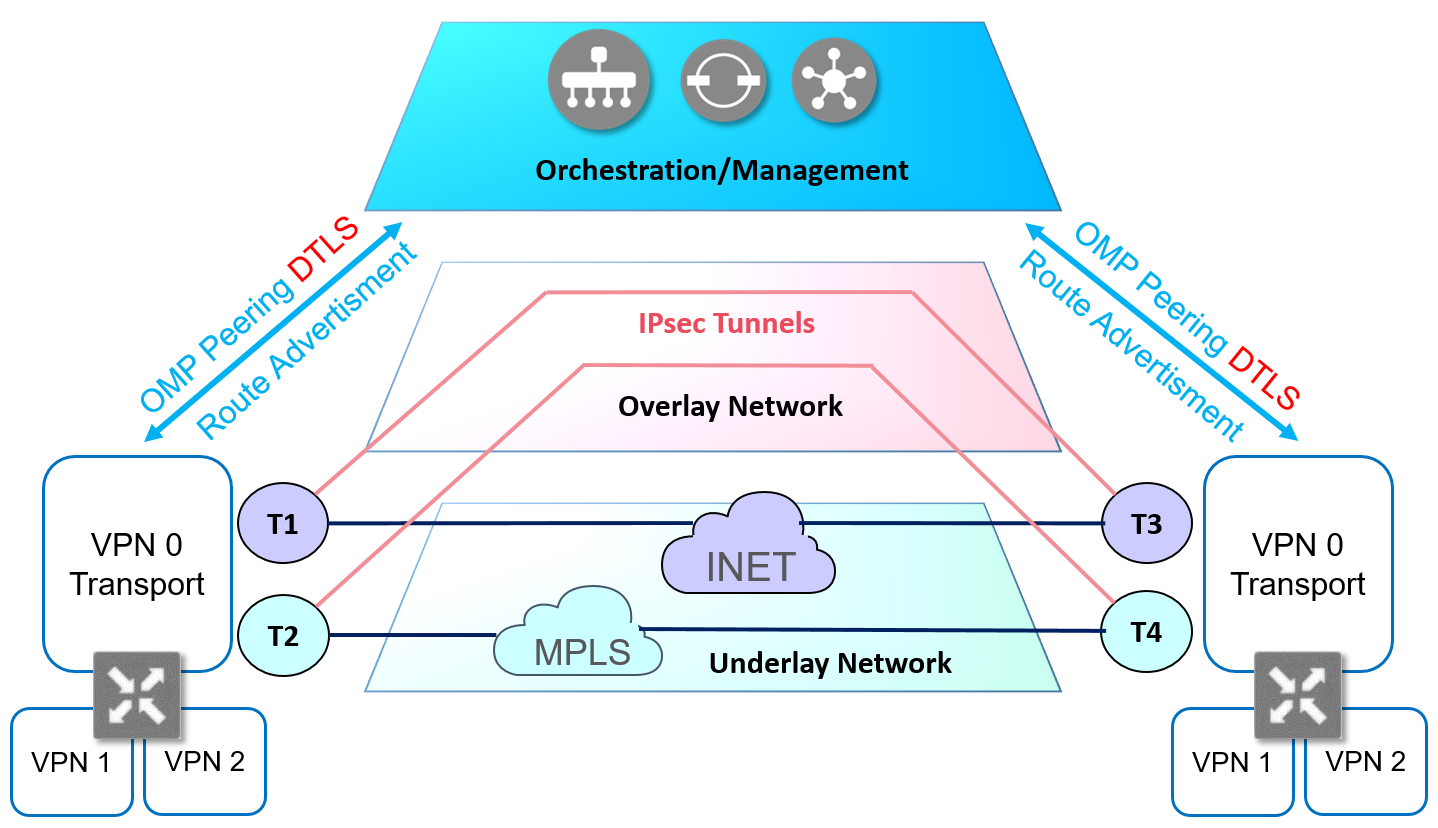
\includegraphics[height=7cm,width=10cm]{../image/Overlay}
	\end{center}
	\caption{Réseau Overlay}
\end{figure} 

Il existe trois types de routes annoncées par OMP :

\begin{itemize}
	\item[$\bullet$]\textbf{  Les routes OMP :} 
	
	Les routes OMP sont utilisées pour l’apprentissage des informations préfixes,ces types de routes peuvent être annoncés dans l'OMP à partir de diverses sources telles que des interfaces connectées, des routes statiques et des protocoles de routage dynamiques tels que OSPF, EIGRP et BGP. Une fois apprises, ces informations de routage sont redistribuées dans le protocole OMP et annoncées au contrôleur vSmart dans la mise à jour OMP.
	Une route OMP Contient les informations suivantes:
	\begin{itemize}
		\item{ Préfixe de destination} 
	\end{itemize}
	\begin{itemize}
		\item{ Préfixe de destination} 
	\end{itemize}
	\begin{itemize}
		\item{ TLOC(Transport Location Identifier):	C’est le prochain saut de la route OMP. Dans le TLOC, il y a trois éléments :
			\begin{itemize}
				\item{ L'adresse IP du système.} 
			\end{itemize}
			\begin{itemize}
				\item{ La couleur: utilisée pour identifier le mode de transport (MPLS ou Internet).} 
			\end{itemize}
			\begin{itemize}
				\item{Le protocole d'encapsulation: peut être GRE ou IPSEC.} 
			\end{itemize}
			\begin{itemize}
				\item{Attributs du préfixe : les attributs tels que l'origine, l'ID de site, le tag, la préférence de chemin et le créateur de la route et l'ID du VPN} 
			\end{itemize}
			
			
\end{itemize}
		
		\newpage
		une route OMP ne sera installée dans la table de transfert du Edge que  si le TLOC next-hop est connu et qu'il existe une session BFD en état actif associée à ce TLOC . La disponibilité des sessions BFD est vérifiée grâce au protocole BFD(Bidirectional Forwarding Detection) qui est un protocole de détection de panne utilisé dans les réseaux informatiques pour détecter rapidement les défaillances de liaison bidirectionnelle entre deux péripheriques de réseau.
	\end{itemize}


	\begin{itemize}
		\item[$\bullet$]\textbf{ Les routes TLOC: } 
	
	
		Une route TLOC (Transport Locator) représente une liaison WAN qui agit comme un point d'extrémité de tunnel dans un environnement SD-WAN. Elle est identifiée de manière unique par trois éléments :
		\begin{itemize}
			\item{ 	Adresse IP système} 
		\end{itemize}
		\begin{itemize}
			\item{ Couleur} 
		\end{itemize}
		\begin{itemize}
			\item{Type d'encapsulation} 
		\end{itemize}
		
		On utilise l'adresse IP système à la place de l'adresse IP de l'interface pour identifier une route TLOC car l'adre sse IP de l'interface peut changer à tout moment, contrairement à l'adresse IP système qui est fixe. Cette stabilité est essentielle car les routes OMP utilisent le next-hop pour pointer vers un TLOC spécifique.De plus ,si un Edge possède plusieurs interfaces de transport connectées à différents fournisseurs WAN, une route TLOC est créée et annoncée pour chaque interface WAN.
		Une route TLOC annonce les attributs d'une terminaison de tunnel SD-WAN, incluant l'encapsulation, la préférence qui est appelée préférence TLOC pour éviter la confusion avec la préférence OMP , l'adresse IP (publique ou privée selon la présence de NAT) et son poids pour la distribution du trafic .
		
	\end{itemize}
	
	\begin{itemize}
		\item[$\bullet$]\textbf{ Les routes de service : } 
		
		Une route de service présente un service réseau, tel qu'un pare-feu ou un équilibreur de charge, connecté à un Edge. Ces services sont souvent déployés dans des endroits centralisés. Le réseau doit être capable de rediriger le trafic depuis n'importe quel site distant à travers ces services, puis de l’acheminer à sa destination initiale.
		La route de service contient les attributs suivants :
		\begin{itemize}
			\item{ ID du VPN  : Le VPN auquel ce service s'applique} 
		\end{itemize}
		\begin{itemize}
			\item{  ID du service: L'identifiant du service définit le type de service annoncé.} 
		\end{itemize}
		\begin{itemize}
			\item{	ID de l'expéditeur : L'adresse IP du Edge qui est à l'origine de la route de service .} 
		\end{itemize}
		\begin{itemize}
			\item{		TLOC : Le TLOC où le service est situé. } 
		\end{itemize}
		
		
	\end{itemize}
	\subsubsection{Réseau Underlay }
	
	Le réseau underlay est l'infrastructure matérielle qui assure la connectivité entre les TLOCs. Sa principale fonction est de permettre le routage selon le next hop, défini par une adresse IP, en utilisant des protocoles de routage traditionnels tels que OSPF, BGP et le routage statique.
	
\subsection{Sécurité}

Les menaces informatiques évoluent et les entreprises ont besoin de solutions de réseau qui offrent une sécurité renforcée. SD-WAN répondent à ce besoin en proposant plusieurs points forts en matière de sécurité.

\subsubsection{Les certificats }
Le SD-WAN s'appuie sur un principe de sécurité qui ne fairt jamais confiance par défaut. C’est à dire chaque Edge qui souhaite participer au réseau doit d'abord s'authentifier et prouver son identité avant d'être autorisé à communiquer.Pour s'authentifier, les Edges utilisent des certificats numériques qui contiennent des informations qui permettent de vérifier l'identité du Edge et de garantir son intégrité.

\subsubsection{Les pare-feu }


Le pare-feu est l'une des formes les plus essentielles de la sécurité des réseaux sur laquelle les organisations s'appuient. 
Cisco a adopté une approche plus moderne en matière de sécurité et a intégré un pare-feu d'entreprise adapté aux applications directement dans les routeurs, éliminant aussi l'extension inutile du réseau sur les sites distants.Prenons l’exemple du Pare-feu applicatif dynamique de type “stateful” qui est capable d’analyser plus de 1400 applications(SD-WAN (3/3) : les 4 avantages principaux de Cisco SD-WAN). Le pare-feu est représenté sous la forme d'une politique de sécurité localisée .Il permet aux équipes de sécurité d'ajouter et de modifier des règles de pare-feu pour des centaines de sites en même temps grâce aux templates et aux fonctions de vManage.  
La séquence d'étapes suivante décrit le mécanisme de configuration de la politique de pare-feu :


\begin{itemize}
	\item{ Définir les zones :une zone source et une zone destination.} 
\end{itemize}
\begin{itemize}
	\item{ Définir une paire de zones : Il est important de définir les paires de zones en tenant compte du sens du trafic prévu.} 
\end{itemize}
\begin{itemize}
	\item{ Créer une politique de sécurité : elle contient toutes les politiques telles que Firewall, IPS, URLF, AMP, etc.}
	\begin{itemize}
		\item{1.Définir une politique de pare-feu.} 
	\end{itemize}
	\begin{itemize}
		\item{ 2.Définir des règles de trafic .} 
	\end{itemize}
	\begin{itemize}
		\item{3.Appliquer la politique de pare-feu à une paire de zones.} 
	\end{itemize}
	
	
\end{itemize}
\begin{itemize}
	\item{ Attacher la politique de sécurité à une template .} 
\end{itemize}

\subsubsection{Les IPS }

Ils dont des systèmes de prévention des intrusions qui analyse le trafic qui circule dans le réseau, Ils utilisent un ensemble de règles prédéfinies, appelées signatures, pour identifier les comportements malveillants.Prenons l’exemple de SNORT qui analyse le trafic réseau en temps réel, ce qui permet de détecter les intrusions et les attaques dès qu'elles se produisent.SNORT travaille en collaboration avec Talos qui fournit des mises à jour automatiques des signatures, ce qui permet de garantir que le système est toujours à jour et capable de détecter les dernières menaces.

\subsubsection{SaSe }
Secure Access Service Edge (SASE) vise à unifier le réseau et la sécurité en une seule solution
Plutôt que de déployer séparément des pare-feu, des systèmes de prévention des intrusions (IPS), des serveurs DNS sécurisés et d'autres outils de sécurité. Cela nous permet de gérer  plus efficacement les politiques de sécurité,de réduire la complexité de l'infrastructure et améliorer la visibilité et le contrôle du réseau.
Le SaSe comporte trois éléments principaux qui travaillent ensemble pour fournir une solution réseau sécurisée et performante pour les entreprises modernes,comme montre la figure. 
\begin{figure} [H]
	\begin{center}
		\centering
		\hspace*{-0.5cm}
		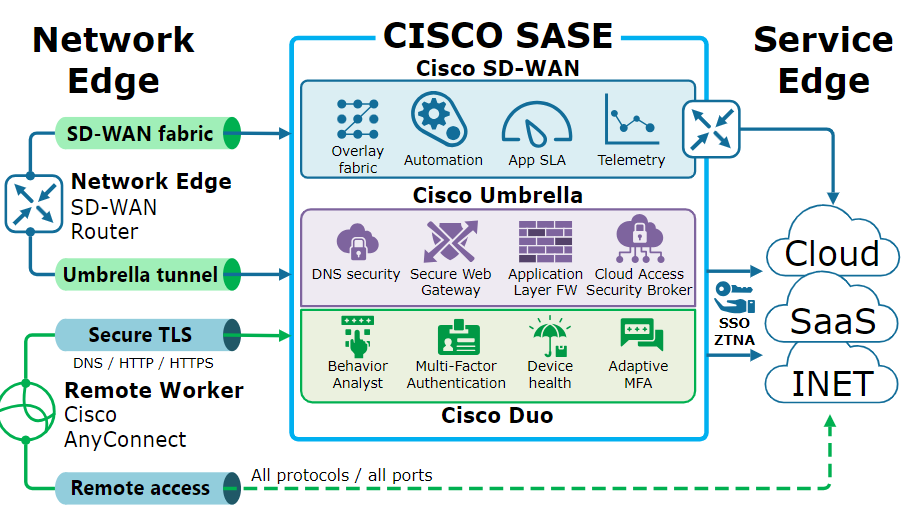
\includegraphics[height=7cm,width=14cm]{../image/sas}
	\end{center}
	\caption{SaSe}
\end{figure} 
\begin{itemize}
	\item[$\bullet$]\textbf{  SD-WAN :} 
	
	Il Gère la connectivité WAN entre les sites et le cloud ,il permet un accès direct à Internet (DIA) dans les sites distants et s'intègre automatiquement avec Umbrella SIG.
\end{itemize}
\begin{itemize}
	\item[$\bullet$]\textbf{ Umbrella SIG(Secure Internet Gateway)  } 
	
	elle fournit une sécurité basée sur le cloud aux utilisateurs distants et remplace les méthodes de sécurité traditionnelles sur site (pare-feu, IPS, proxy).Elle peut aussi combiner plusieurs fonctions de sécurité ,pare-feu cloud, une passerelle web sécurisée (SWG), une inspection de la couche DNS, un courtier de sécurité d'accès en nuage (CASB), une prévention de la perte de données (DLP) et une isolation du navigateur à distance (RBI) en un seul service fourni en nuage qui s'intègre de manière transparente avec le SD-WAN.
\end{itemize}
\begin{itemize}
	\item[$\bullet$]\textbf{ Duo Network Gateway (DNG)} 
	Il fournit un accès sécurisé aux ressources internes pour les utilisateurs distants et élimine la nécessité de gérer les identifiants VPN.De plus il ajoute une couche supplémentaire de sécurité avec l'authentification multifacteur (MFA) et permet un contrôle d'accès granulaire par application et par groupe d'utilisateurs ce qui garantit que seuls les utilisateurs et les appareils autorisés peuvent accéder aux ressources internes.
\end{itemize}
\section{Les Composantes du Cisco Viptela SD-WAN  }

Le SD-WAN de Cisco Viptela s'appuie sur divers éléments, comme illustré dans la figure , qui collaborent pour offrir une solution robuste et solide.
\begin{figure} [H]
	\begin{center}
		\centering
		\hspace*{-0.5cm}
		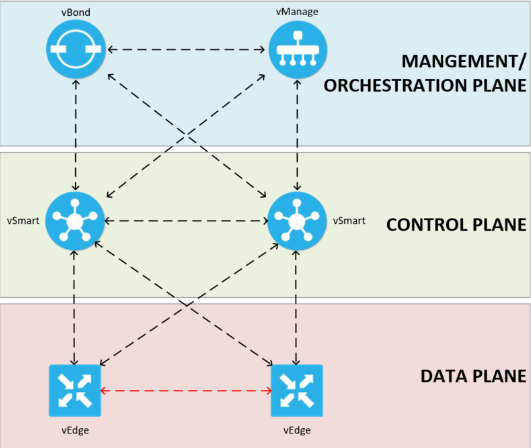
\includegraphics{../image/composantes}
	\end{center}
	\caption{Les Composantes du Cisco Viptela SD-WAN }
\end{figure} 


\subsection{vManage}

vManage est le point de contrôle central dans l'infrastructure SD-WAN. Il offre une interface centralisée pour la configuration, la gestion et la surveillance du réseau. Les administrateurs peuvent établir des politiques de routage, des règles de sécurité, ainsi que diagnostiquer et surveiller les performances du réseau via son tableau de bord.

\subsection{vBond }

vBond agit comme un orchestrateur au sein de l'infrastructure Cisco SD-WAN. Il détermine la construction du réseau et partage ces informations avec les autres composants. C'est le premier point d'accès et d'authentification pour les équipements SD-WAN intégrés à l'overlay (structure logique) , il conserve la liste de tous les équipements autorisés à rejoindre l'overlay SD-WAN. En outre, vBond facilite le Traversal NAT (NAT-T) au sein de l'architecture SD-WAN. La provision sans intervention et la diffusion des données de contrôle et de gestion font  partie des responsabilités assurées par Cisco vBond.

\subsection{vSmart }
vSmart est le composant clé du plan de contrôle dans l'architecture SD-WAN de Cisco. Il est le cerveau des solutions, Il collecte des informations sur l'état du réseau, les politiques de routage et les performances des liaisons. En fonction de ces données, le vSmart prend des décisions de routage intelligentes et distribue les politiques aux autres périphériques du réseau. L'échange d'informations de routage se fait via le contrôleur vSmart et non directement avec les autres sites distants. Vsmart  agit  aussi comme un "route reflector" dans le monde BGP en annonçant ou en filtrant les routes de l’overlay Cisco SD-WAN aux routeurs Edges.
\subsection{Les Edges }

Ils existent plusieurs périphériques dans Cisco SD-WAN Viptela. Ils jouent des rôles spécifiques dans l'architecture du sdwan avec une différence dans leur emplacement de déploiement et leur optimisation pour des environnements particuliers.
\subsubsection{   vEdge  (Virtual Edge) }

Le vEdge est un périphérique de bordure SD-WAN déployé sur site, il peut être  dans un datacenter ou un environnement cloud. Il agit comme un point d'entrée et de sortie pour le trafic en  assurant son acheminement entre les différents sites distants et en  établissant des tunnels sécurisés pour garantir la connectivité avec les autres périphériques vEdge. Il communique avec le vSmart et le vBond pour le contrôle et l'orchestration du réseau, tout en assurant le chiffrement des données pour protéger les communications.

\subsubsection{  cEdge  (Cloud Edge) }


Le cEdge fonctionne de manière similaire au vEdge,il est déployé dans des environnements cloud publics tels que AWS, Azure ou Google Cloud Platform, afin d'assurer une connectivité SD-WAN optimisée au cloud via des tunnels sécurisés.De plus,il est Capable de s'intégrer avec les services cloud natifs pour améliorer les performances et l'efficacité.




\section*{Conclusion }

Dans ce chapitre, nous avons exploré en détail le Cisco Viptela SD-WAN, Nous avons examiné en profondeur son architecture, ses fonctionnalités et ses composants. Dans le prochain chapitre, nous allons voir  la mise en œuvre pratique de la solution, en décrivant les étapes nécessaires pour déployer et configurer le Cisco Viptela SD-WAN dans un environnement réel.


	%	\input{Chaps/Conc-gene.tex}
		%\bibliographystyle{unsrt}
		%\raggedright
		%\bibliography{Bib/references.bib}
\end{document}